\newpage
\section{Auswertung}
\label{sec:Auswertung}

Zur Optimierung des FID werden folgende Parameter gewählt:
\begin{align}
&\text{Phase:} & \phi&= \SI{111}{\degree}\\
&\text{Pulslänge:} & t_{\SI{90}{\degree}}& =  \SI{4.74}{\micro\second}\\
&\text{Resonanzfrequenz:} & f_{\text{res}}&= \SI{21.71575}{\mega\hertz}\\
&\text{Shim-Parameter:} & x&=\num{-2.02} & y&=\num{-5.24} & z&=\num{3.68} & z^2&=\num{-2.74}
\end{align}

\subsection{Bestimmung der Relaxationszeit $T_{2}$ mit der Meiboom-Gill-Methode}
\label{subsec:T2}
Um die Relaxationszeit $T_{2}$ zu bestimmen, werden die Signale, der mit dem Oszilloskop aufgenommenen
Burst-Sequenz der Meiboom-Gill Methode(siehe Abbildung \ref{fig:meiboomgill} und \ref{fig:t2_gesamt}) gegen die Zeit aufgetragen.
Zusätzlich wird eine Burst-Sequenz der Carr-Pucell Methode(siehe Abbildung \ref{fig:carrpucell}) aufgenommen, in der die
Problematik eines zu kurzen/langen $\SI{180}{\degree}$-Pulses deutlich wird, da
sich die Fehler bei der Carr-Pucell Mehtode aufsummieren.
Die Amplitude fällt deshalb schneller als bei der Meibomm-Gill Methode
ab und liefert ein zu kleines $T_2$.
Um die Echoamplituden aus der Meilbomm-Gill-Sequenz zu finden, werden
zunächst Werte, deren Betrag unterhalb von \SI{0.02}{\volt} liegen, herausgefiltert.
Anschließend werden jeweils in einer Umgebung von $20$ Messwerten, lokale
Maxima gesucht.
In Tabelle \ref{tab:t2_fitwerte}
sind die auf diese Weise gefundenen Echos angegeben.
Anschließend wird für den in Gleichung \eqref{eqn:t2} gegebenen Zusammenhang unter \textit{Python3} mit Hilfe der Funktion \textit{curvefit} aus
dem Paket \textit{Scipy} eine Regression der als Echos identifizierten Messwerte durchgeführt.\\
Dabei ergeben sich für den Startwert $U_{0}$ und Relaxationszeit $T_{2}$ die folgenden Werte
\begin{align*}
  U_{0} &= \SI{0.90+-0.04}{\volt} \\
  T_{2} &= \SI{1.49+-0.08}{\second} \, .
\end{align*}
In Abbildung \ref{fig:t2_plot} sind die verwendeten Messwerte, sowie der Graph der zugehörigen Regression
gezeigt.\\


\begin{figure}[hhh]
  \centering
  \includegraphics[width=0.7\textwidth]{build/t_u_plot2_extrem.pdf}
  \caption{Verwendete Messwerte(Signal logarithmiert) für $T_{2}$ Messung mit Meiboom-Gill-Methode, sowie zugehörige Regression.}
  \label{fig:t2_gesamt}
\end{figure}


\begin{figure}[hhh]
  \centering
  \includegraphics[width=0.7\textwidth]{build/t_u_plot2.pdf}
  \caption{Aufgenommene Messwerte für $T_{2}$ Messung mit Meiboom-Gill-Methode.}
  \label{fig:t2_plot}
\end{figure}


\begin{figure}[hhh]
  \centering
  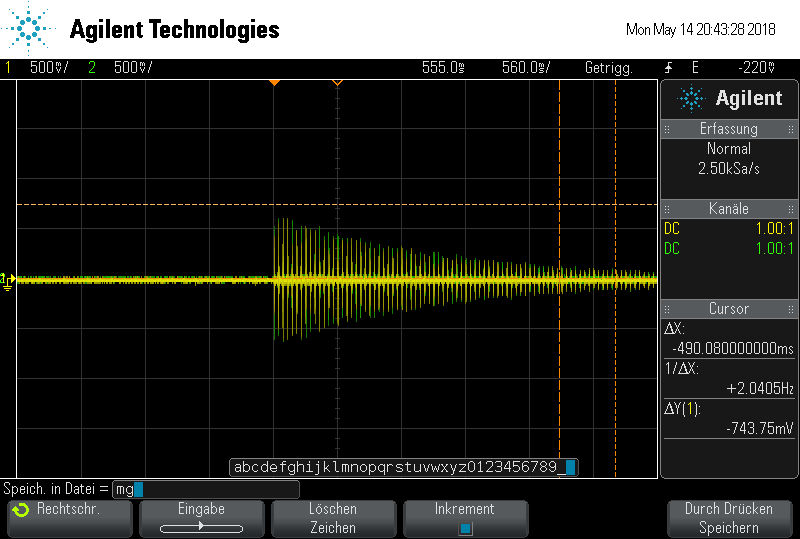
\includegraphics[width=0.7\textwidth]{mg.png}
  \caption{Messwerte für $T_{2}$ Messung mit Meiboom-Gill-Methode(Bild am Oszilloskop).}
  \label{fig:meiboomgill}
\end{figure}

\begin{figure}[hhh]
  \centering
  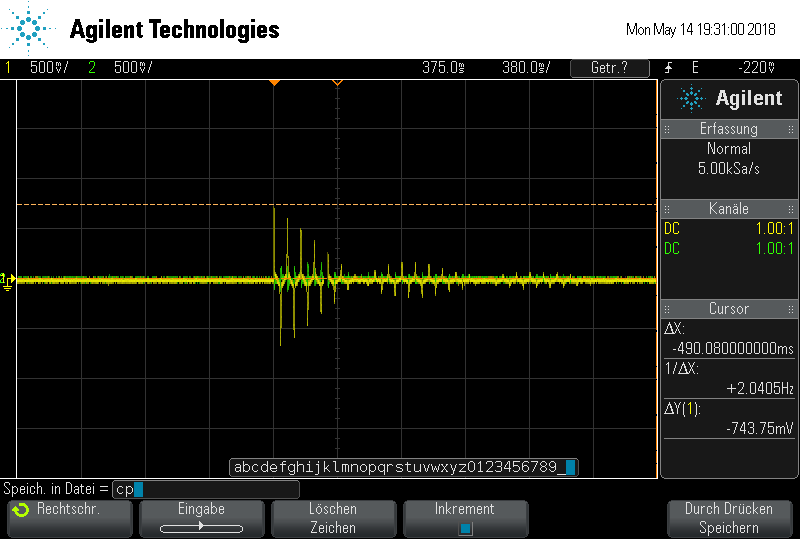
\includegraphics[width=0.7\textwidth]{cp.png}
  \caption{Messwerte für $T_{2}$ Messung mit Carr-Purcell-Methode(Bild am Oszilloskop).}
  \label{fig:carrpucell}
\end{figure}


Der Literaturwert\cite{litwerte} für die Relaxationszeit $T_{2}$ von bidestilliertem Wasser
beträgt
\begin{align*}
  T_{2}^\text{lit.} = \SI{1.52+-0.093}{\second},
\end{align*}
sodass sich eine relative Abweichung $f$ des experimentell bestimmten Werts
von
\begin{align*}
  f = \frac{T_{2} - T_{2}^\text{lit.}}{T_{2}^\text{lit.}} = \SI{2+-8}{\percent}
\end{align*}
ergibt.


\begin{table}
  \centering
  \caption{Gefundene Echos für die Bestimmung der Relaxationszeit $T_{2}$.}
  \label{tab:t2_fitwerte}
  \begin{tabular}{c c| c c}
  \toprule
  $t \text{ in } \si{\milli\second}$ & $U \text{ in } \si{\milli\volt}$ &  $t \text{ in } \si{\milli\second}$ & $U \text{ in } \si{\milli\volt}$\\

\midrule
669.2	&	561.56  & 2388.4	&	159.55  \\
949.2	&	501.26  & 2668.4	&	119.35  \\
1349.6	&	380.65 & 3228.4	&	119.35   \\
1548.4	&	280.15 & 3869.6	&	79.15    \\
1789.2	&	280.15 & 4309.2	&	40.20    \\
1909.6	&	280.15 & 4628.4	&	59.04    \\
2150.4	&	219.85 & &  \\
  \bottomrule
  \end{tabular}
\end{table}


\FloatBarrier
\subsection{Bestimmung des Diffusionskoeffizienten mit der Spin-Echo-Methode}
\label{subsec:D}
Der Diffusionskonstante wird aus den in Tabelle \ref{tab:diffusion} angegebenen
Messwerten bestimmt.
Dazu wird eine Regression der Werte für den in Gleichung \eqref{eqn:32} gegebenen Zusammenhang mit
\textit{curvefit} durchgeführt.
Als Fitparameter werden der Vorfaktor $a$ sowie die Diffusionskonstante gewählt. Für $T_{2}$ wird der in Abschnitt
\ref{subsec:T2} bestimmte Wert verwendet. Der Gradient $G$ wird aus dem Zusammenhang
\begin{align}
  \label{eqn:gradient}
  G = \frac{8.8}{d \, \gamma \, t_{\frac{1}{2}}}
\end{align}
gewonnen. Dabei bezeichnet $d$ den Probendurchmesser, von $\SI{4.4}{\milli\meter}$, $\gamma$ das gyromagnetische Verhältnis
von Protonen in Wasser und $t_{\frac{1}{2}}$ die Halbwertszeit des Echos.
Wird der Ausdruck \eqref{eqn:gradient} in Gleichung \eqref{eqn:32} eingesetzt, ist leicht zu erkennen, dass $\gamma$ wegfällt und
nur noch $d$ und $t_{\frac{1}{2}}$ eingesetzt werden müssen.
Da in Gleichung \eqref{eqn:32} die Zeit $t$ verwendet wird, allerdings $\tau$ gemessen wurde, müssen
die gemessenen Werte für die Zeit noch gemäß
\begin{align}
  t = 2 \tau
\end{align}
umgerechnet werden.
Für die Halbwertsbreite wurde kein Wert gemessen.
Daher wird zunächst ein Fit der Form
\begin{align}
  M(t) = \alpha \, e^{-\frac{t}{T_{2}}} \, e^{-\beta t^{3}}
\end{align}
an die Messwerte vorgenommen.
Aus dem Parameter $\beta$ kann über
\begin{align}
  t_{\frac{1}{2}} = \sqrt{\frac{8.8^{2} D_{\text{lit}}}{12 \, \beta d^{2} } }
\end{align}
die Halbwertsbreite bestimmt Werden.
Für die Parameter $\alpha$ und $\beta$ ergeben sich
\begin{align*}
  \alpha &= \SI{0.751+-0.006}{\volt}\\
  \beta &= \SI{5196.12+-161.33}{\per\second\cubed} \, .
\end{align*}
Für die Halbwertszeit ergibt sich grob
\begin{align*}
  t_{\frac{1}{2}} = \SI{355+-6}{\micro\second}.
\end{align*}
Mit dem bestimmten Wert für die Halbwertsbreite wird nun die Regression zur Bestimmung der Diffusionskonstanten durchgeführt.
In Abbildung \ref{fig:diffusion} sind die Messwerte, sowie der Graph der Regression dargestellt.\\
Als Regressionsparameter ergeben sich
\begin{align*}
  a &= \SI{0.751+-0.006}{\volt}\\
  D &= \SI{1.97+-0.54 e-9}{\meter\squared\per\second} \, .
\end{align*}

Der Literaturwert \cite{wang1965self} für die Diffusionskonstante bei der Temperatur
$\SI{25}{\celsius}$ ist
\begin{align*}
  D^\text{lit.} = \SI{1.97+-0.06 e-9}{\meter\squared\per\second} \, ,
\end{align*}
sodass die relative Abweichung $f$ des experimentell bestimmten Werts
vom Theoriewert
\begin{align*}
  f = \frac{T_{1} - T_{1}^\text{lit.}}{T_{1}^\text{lit.}} = \SI{0.00(3)}{}
\end{align*}


\begin{table}
  \centering
  \caption{Verwendete Messwerte für die Bestimmung der Diffusionskonstanten.}
  \label{tab:diffusion}
  \begin{tabular}{c c}
  \toprule
  $t \text{ in } \si{\milli\second}$ & $U \text{ in } \si{\milli\volt}$\\
  \midrule
  0.0	&	793.75   \\ 
5.0	&	750.00   \\ 
10.0	&	737.50   \\ 
15.0	&	718.75   \\ 
20.0	&	700.00   \\ 
25.0	&	675.00   \\ 
30.0	&	634.75   \\ 
35.0	&	593.75   \\ 
40.0	&	500.00   \\ 
45.0	&	443.75   \\ 
50.0	&	387.50   \\ 
55.0	&	306.25   \\ 
60.0	&	243.75   \\ 
65.0	&	181.25   \\ 

  \bottomrule
  \end{tabular}
\end{table}


\begin{figure}[hhh]
  \centering
  \includegraphics[width=0.7\textwidth]{build/t_u_plotdiff.pdf}
  \caption{Messwerte für die Bestimmung des Diffusionskoeffizienten, sowie zugehörige Regression.}
  \label{fig:diffusion}
\end{figure}

\FloatBarrier
\subsubsection{Bestimmung der Viskosität}
\label{subsubsec:viskositaet}
Die Viskosität von Wasser wird mit Hilfe eines Viskosimeters bestimmt.
Am Viskosimeter werden zwei Zeiten gemessen
\begin{align*}
  t_{1}^\text{visk.} &= \SI{723.5+-2}{\second}\\
  t_{2}^\text{visk.} &= \SI{720.3+-2}{\second}\, .
\end{align*}
Es wird mit dem Mittelwert der beiden Zeiten
\begin{align*}
  t^\text{visk.} &= \SI{721.9+-1.4}{\second}
\end{align*}
gerechnet.\\
Um aus der gemessenen Zeit die Viskosität zu bestimmen wird der Zusammenhang
\begin{align}
  \eta = a \left(t - \delta \right)
\end{align}
verwendet. Dabei bezeichnet $a$ eine Apparaturkonstante die mit $a = \SI{1.024e-9}{}$ angegeben wird und $\delta$
eine Apparaturkonstante die mit $\delta = \SI{0.8562+-0.0014}{}$ angegeben wird.
Für die Viskosität ergibt sich auf diese Weise
\begin{align*}
  \eta = \SI{0.7364+-0.0014 e-3}{\meter\squared\per\second} \, .
\end{align*}

% weglassen?
Der Literaturwert\cite{litvisk} für die Viskosität bei einer Temperatur von $\SI{25}{\celsius}$ ist
\begin{align*}
  \eta^\text{lit.} = \SI{0.891e-3}{\meter\squared\per\second} \, ,
\end{align*}
sodass die relative Abweichung $f$ des experimentell bestimmten Werts
vom Theoriewert
\begin{align*}
  f = \frac{\eta - \eta^\text{lit.}}{\eta^\text{lit.}} = \SI{17.4+-0.2}{\percent}
\end{align*}


\FloatBarrier
\subsubsection{Bestimmung des Molekülradius}
\label{subsubsec:molekuelradius}
Mit bekanntem Diffusionskoeffizienten $D$ und Viskosität $\eta$
und bei einer Temperatur $T=\SI{25}{\celsius}$
kann gemäß
der Stokesschen Formel folgender Zusammenhang für den Molekülradius $R$ hergeleitet werden
\begin{align}
  \label{eqn:stokes}
  R = \frac{k_\text{B} \, T}{6 \pi \, \eta \, D} \, .
\end{align}
Mit den vorher bestimmten Werten ergibt sich für den Molekülradius
\begin{align*}
  R = \SI{1.51(5)}{\angstrom} \, .
\end{align*}
Dieser Wert soll nun verglichen werden, mit einem Molekülradius, der ermittelt werden kann,
indem angenommen wird, dass sich
Kugelförmige Wassermoleküle in einer hexagonal dichtesten Packung anordnen
und einem Molekülradius, der sich durch die Annahme ergibt, dass sich das Wasser als eines van-der-Waals-Gas
beschreiben lässt.
Für die erste Annahme ergibt sich ein Radius von
\begin{align*}
  R_{\text{hexagonal}} = \sqrt{\frac{m}{4\sqrt{2} \, \rho}} \, .
\end{align*}
Wobei $\rho=\SI{997.2995}{\kilo\gram\per\meter\tothe{3}}$  \cite{litdicht} die Dichte von Wasser bei Raumtemperatur $T=\SI{24}{\celsius}$
und $m=\SI{29.915e-27}{\kilo\gram}$ \cite{litatomgewicht} das Atomgewicht von Wasser bezeichnet.
Mit diesem Zusammenhang ergibt sich
\begin{align*}
  R_{\text{hexagonal}} = \SI{1.744}{\angstrom}.
\end{align*}
Für die zweite Annnahme ergibt sich ein Radius von
\begin{align}
R_{\text{van-der-Waal}}= \left(\frac{3b}{16\pi N_A}\right)^{\frac{1}{3}},
\end{align}
da das Kovolumen $b$ ungefähr das
vierfache des Eigenvolumen eines Moleküle ist.
Für Wasser mit $b=\SI{31e-6}{\meter\tothe{3}\per\mol}$ \cite{litwaal} ergibt sich ein Radius von
\begin{align}
R_{\text{van-der-Waal}}= \SI{1.454}{\angstrom}.
\end{align}

\subsubsection{Bestimmung der Relaxationszeit $T_{1}$}
\label{subsubsec:T1}
Zur Bestimmung der Relaxationszeit $T_{1}$ werden die in Tabelle \ref{tab:t1} angegebenen
Messwerte verwendet und in Abbildung \ref{fig:T_1bestimmung} gegeneinander aufgetragen.
Um $T_{1}$ aus Gleichung \eqref{eqn:33} zu bestimmen wird eine Regression
mit der Funktion
\begin{align}
  \label{eqn:t1_bestimmung}
  a \, \left( 1 - 2 e^{-\frac{\tau}{T_{1}}} \right)
\end{align}
der Messwerte vorgenommen. In Abbildung \ref{fig:T_1bestimmung} ist
der mit Hilfe der Regression erzeugte Funktionsgraph dargestellt.
Somit lässt sich $T_{1}$ aus den Regressionsparameter
\begin{align*}
  a &= \SI{0.7628+-0.0048}{}\\
  T_{1} &= \SI{2.3328+-0.0296}{}
\end{align*}
entnehmen.
Es ergibt sich sich für die gesuchte Relaxationszeit
\begin{align*}
  T_{1} = \SI{2.33+-0.03}{\second} \, .
\end{align*}


Der Literaturwert\cite{litwerte} für die bestimmte Relaxationszeit ist
\begin{align*}
  T_{1}^\text{lit.} = \SI{3.09+-0.15}{\second} \, ,
\end{align*}
sodass die relative Abweichung $f$ des experimentell bestimmten Werts
vom Theoriewert
\begin{align*}
  f = \frac{T_{1} - T_{1}^\text{lit.}}{T_{1}^\text{lit.}} = \SI{25+-4}{\percent}
\end{align*}


\begin{figure}[hhh]
  \centering
  \includegraphics[width=0.7\textwidth]{build/t_u_plott1.pdf}
  \caption{Messwerte für die Bestimmung der Relaxationszeit $T_{1}$, sowie zugehörige Regression.}
  \label{fig:T_1bestimmung}
\end{figure}


\begin{table}
  \centering
  \caption{Verwendete Messwerte für die Bestimmung der Relaxationszeit $T_{1}$.}
  \label{tab:t1}
  \begin{tabular}{c c|}
  \toprule
  $t \text{ in } \si{\milli\second}$ & $U \text{ in } \si{\milli\volt}$\\
  \midrule
  0.5	&	-818.75   \\
  1.0	&	-800.00   \\
  1.5	&	-793.75   \\
  2.0	&	-787.50   \\
  2.5	&	-787.50   \\
  3.0	&	-800.25   \\
  3.5	&	-787.50   \\
  4.0	&	-781.25   \\
  4.5	&	-775.00   \\
  5.0	&	-768.75   \\
  5.5	&	-762.50   \\
  10.0	&	-756.25   \\
  15.0	&	-762.50   \\
  30.0	&	-750.00   \\
  60.0	&	-731.25   \\
  100.0	&	-693.75   \\
  120.0	&	-681.25   \\
  180.0	&	-643.75   \\
  240.0	&	-587.50   \\
  300.0	&	-550.00   \\
  360.0	&	-518.75   \\
  420.0	&	-481.25   \\
  \bottomrule
  \end{tabular}
  \begin{tabular}{|c c}
  \toprule
  $t \text{ in } \si{\milli\second}$ & $U \text{ in } \si{\milli\volt}$\\
  \midrule
  500.0	&	-443.75   \\
  600.0	&	-381.25   \\
  700.0	&	-325.00   \\
  800.0	&	-287.50   \\
  900.0	&	-243.75   \\
  1000.0	&	-206.25   \\
  1100.0	&	-181.25   \\
  1200.0	&	-143.75   \\
  1300.0	&	-112.50   \\
  1400.0	&	-75.00   \\
  1500.0	&	-68.75   \\
  2000.0	&	106.25   \\
  2500.0	&	218.75   \\
  3000.0	&	312.50   \\
  3500.0	&	406.25   \\
  4000.0	&	481.25   \\
  5000.0	&	550.00   \\
  6000.0	&	606.25   \\
  7000.0	&	662.50   \\
  8000.0	&	700.00   \\
  9000.0	&	725.00   \\
  9999.0	&	743.75   \\
  \bottomrule
  \end{tabular}
\end{table}


% \begin{figure}
%   \centering
%   \includegraphics[width=0.7\textwidth]{plot.pdf}
%   \caption{Plot.}
%   \label{fig:plot}
% \end{figure}
